
\documentclass[10pt]{beamer}
% \usepackage{subfiles}

\usepackage[danish]{babel}
\usepackage[utf8]{inputenc}
\usetheme[progressbar=frametitle]{metropolis}
\usepackage{appendixnumberbeamer}


\usepackage{booktabs}
\usepackage[scale=2]{ccicons}

% \usepackage{pgfplots}
% \usepgfplotslibrary{dateplot}

\definecolor{Orange}{RGB}{229,134,25}

\usepackage{xspace}
\newcommand{\themename}{\textbf{\textsc{metropolis}}\xspace}
\usepackage{listings}


\definecolor{background}{RGB}{226, 226, 226}


\lstset{ 
literate=% 
{Ö}{{\"O}}1 
{Ä}{{\"A}}1 
{Ü}{{\"U}}1 
{ß}{{\ss}}{ 1\negmedspace\,} 
{ü}{{\"u}}1 
{ä}{{\"a}}1 
{ö}{{\"o}}1 
{ø}{{\o}}{1\negmedspace\,} 
{Ø}{{\O}}{1\negthinspace\,\,} 
{å}{{\aa}}{1\negthickspace\,} 
{Å}{{\AA}}{1\negthinspace\;} 
{æ}{{\ae}}{1\negthinspace\;} 
{Æ}{{\AE}}{1\,\,}}

\lstdefinestyle{terminal}{
	language=bash,
	aboveskip=2mm,
	belowskip=2mm,
	showstringspaces=false,
	columns=flexible,
	basicstyle={\small\ttfamily},
	numbers=none,
	numberstyle=\footnotesize,
	commentstyle=\color{black},
	frame=single,
	framesep=2pt,
	breaklines=true,
	breakatwhitespace=false,
	backgroundcolor = \color{background},
	tabsize=2
}


\lstdefinestyle{python}{
	language=Python,
	aboveskip=2mm,
	belowskip=1mm,
	showstringspaces=false,
	columns=flexible,
	numbers=none,
	numberstyle=\footnotesize,
	commentstyle=\ttfamily\color{black},
	frame=single,
	framesep=2pt,
	breaklines=true,
	breakatwhitespace=false,
	backgroundcolor = \color{background},
	tabsize=2
}



\title{Lær Python dag 1 - modul 1}
\subtitle{Introduktion, basis python}
% \date{\today}
\date{}
\author{Steffen Berg Klenow \\Jonas Bamse Andersen}
\institute{Syddansk Universitet}
% \titlegraphic{\hfill\includegraphics[height=1.5cm]{logo.pdf}}


\title{Lær Python dag 1 - modul 1}
\subtitle{Introduktion, basis python}

\begin{document}

\maketitle

\begin{frame}{Indhold}
  \setbeamertemplate{section in toc}[sections numbered]
  \tableofcontents[hideallsubsections]
\end{frame}

\section{Velkommen}

\begin{frame}[fragile]{Hvem er vi}
	\begin{columns}
		\column{0.4\textwidth}
			\begin{center}
				\includegraphics[width=0.5\textwidth]{figures/steffen.jpg}
			\end{center}
			Steffen Berg Klenow
			\begin{itemize}
				\item 23 år
				\item Datalogi 7. semester
				\item Fritid: Foto og cykling
			\end{itemize}
		\column{0.4\textwidth}
			\begin{center}
				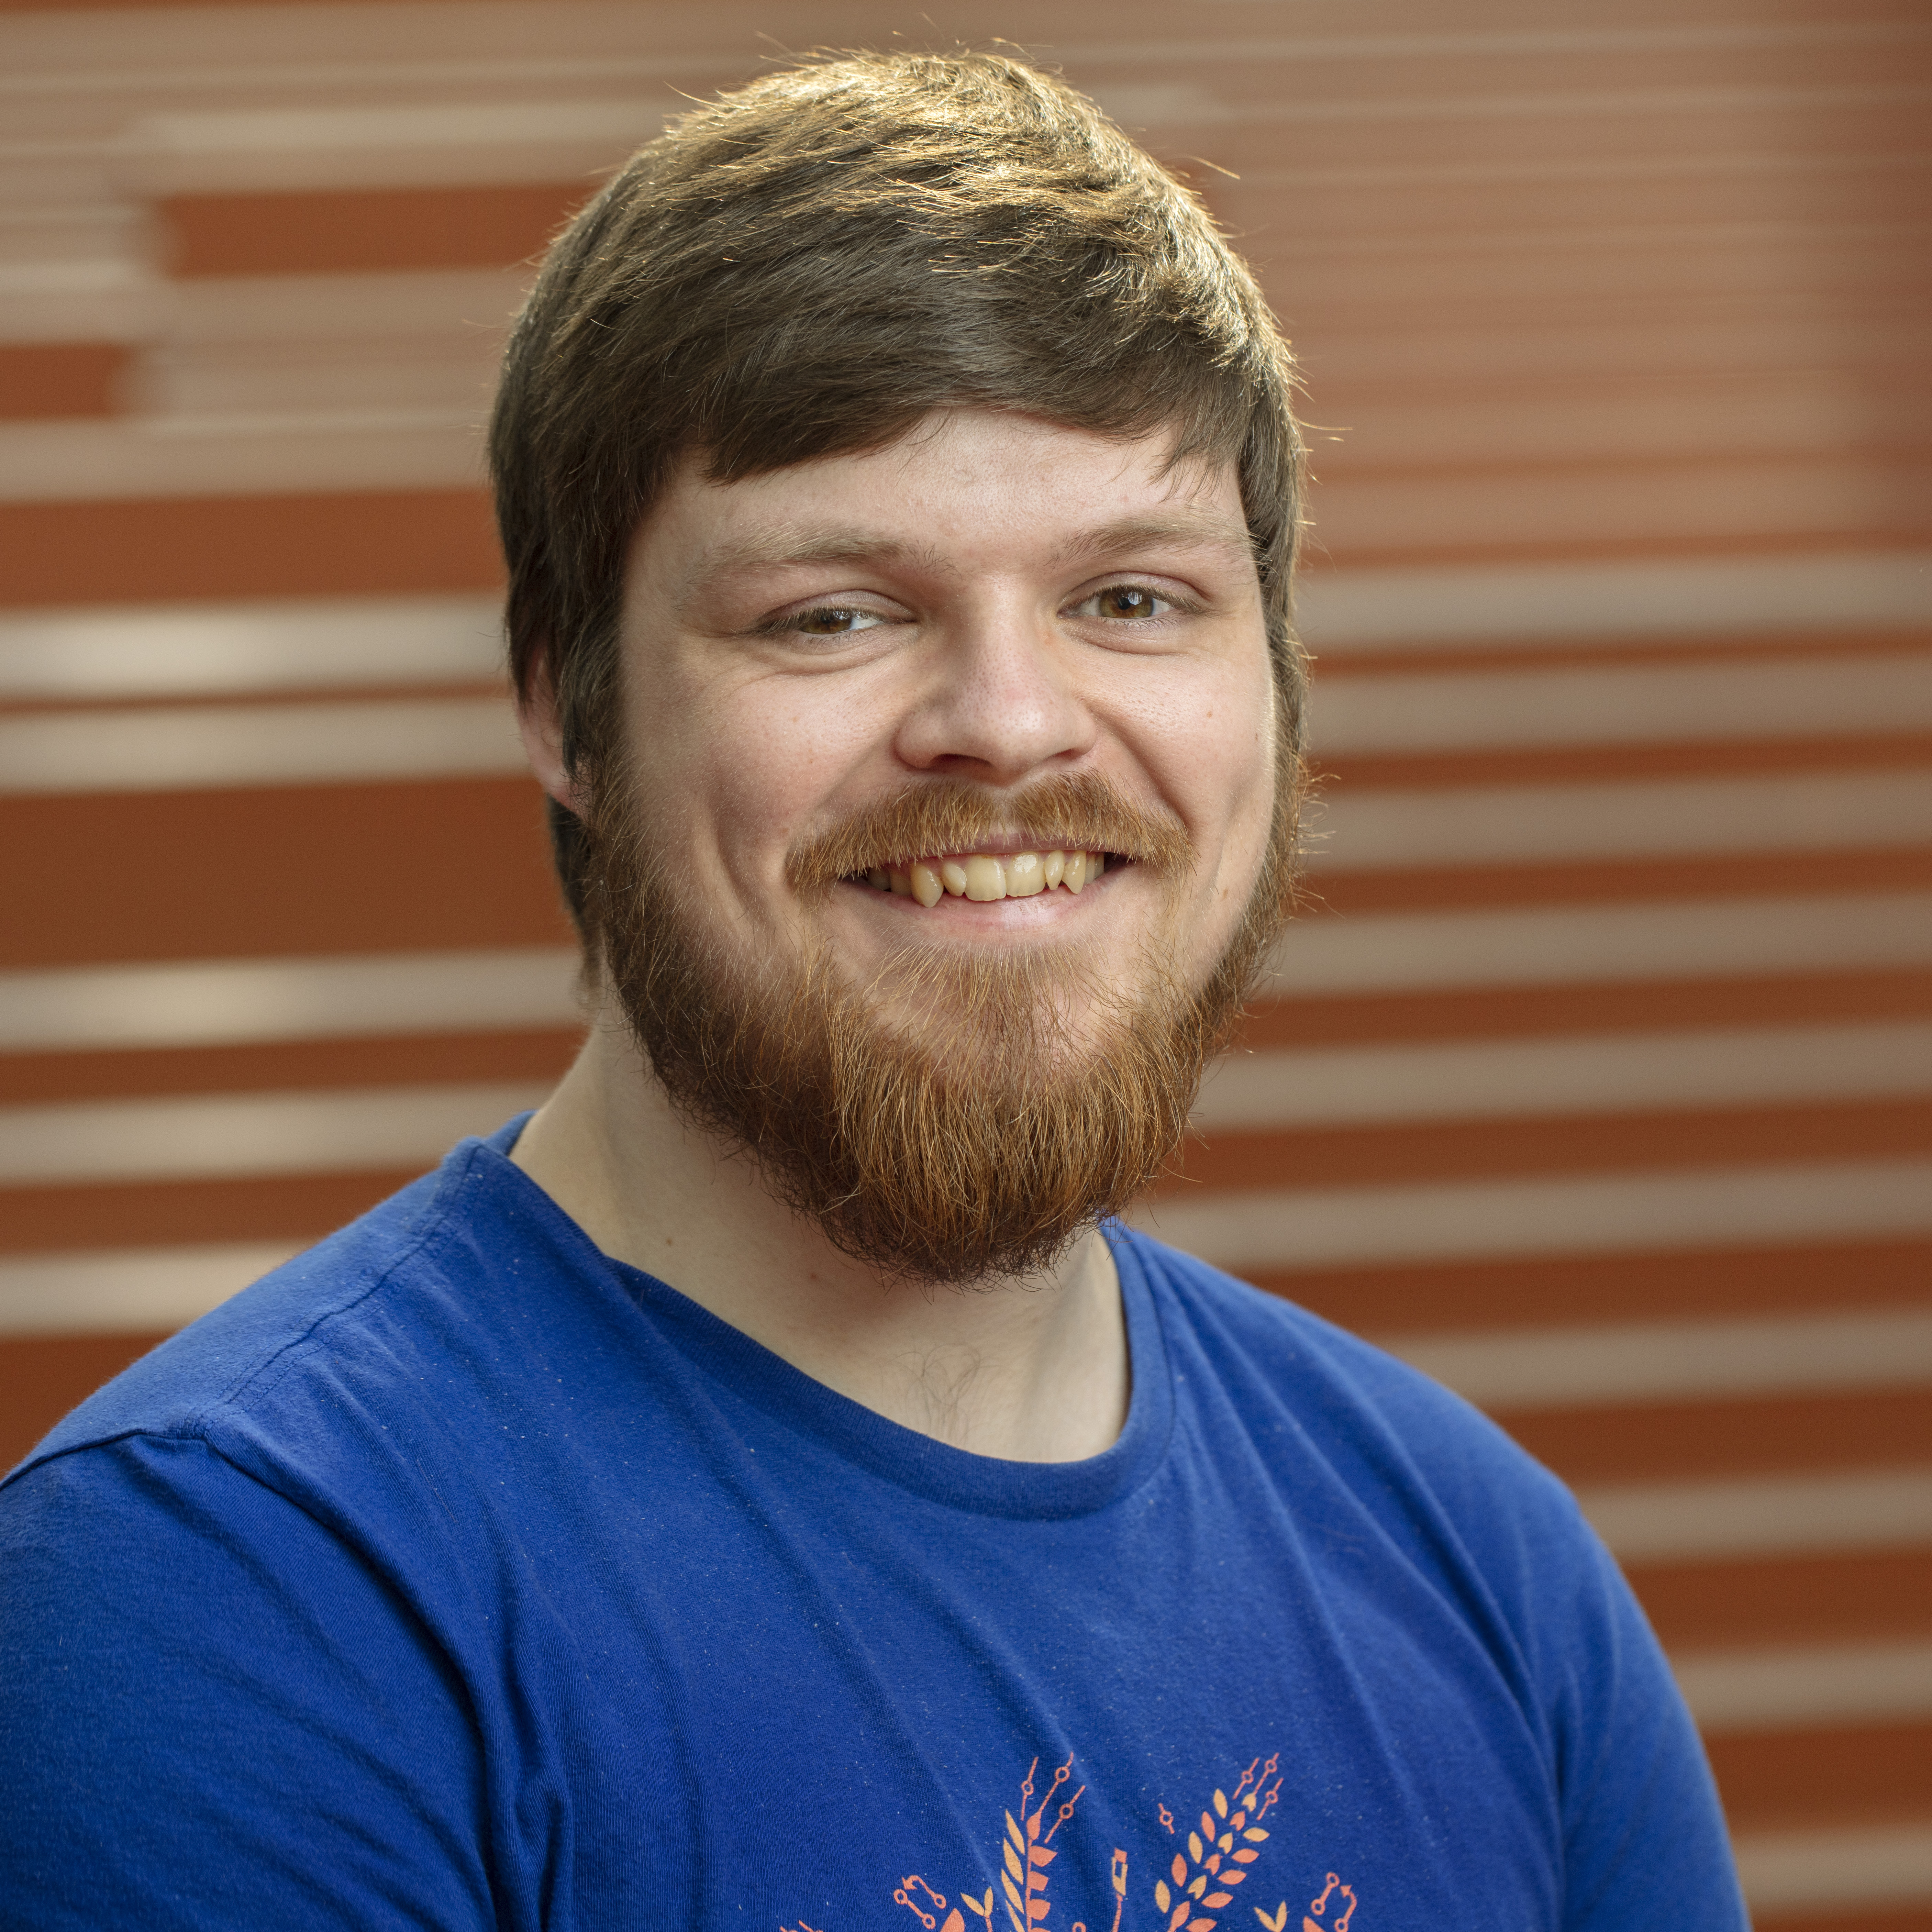
\includegraphics[width=0.5\textwidth]{figures/bamse.jpg}
			\end{center}
			Jonas Bamse Andersen
			\begin{itemize}
				\item 23 år
				\item Datalogi 7. semester
				\item Fritid: FDF og gaming
			\end{itemize}
	\end{columns}
\end{frame}

\begin{frame}[fragile]{Kursets Opbygning}
	To moduler pr dag, pause/frokost imellem modulerne\\
	Et modul består af:
	\begin{itemize}
		\item Introduktion
		\item Opgaver
	\end{itemize}
	\vfill
	Learn by doing. Tag små pauser når I har brug for det.\\
	Husk at stille spørgsmål!
\end{frame}

\begin{frame}[fragile]{Hjemmeside}
	\begin{center}
		\includegraphics[width=0.8\textwidth]{figures/hjemmeside.png}
	\end{center}
	Kurset har en hjemmeside: \url{https://imada.sdu.dk/~sklen15/python/}

	Her findes slides, opgaver og eventuelle tips og tricks.	
\end{frame}

\begin{frame}{Software}
	Python og en tekst-editor skal installeres.
	\begin{itemize}
		\item Python 3.7
		\item Editor/IDE: Sublime, Visual Studio Code, Pycharm...
	\end{itemize}
	\begin{center}
		\includegraphics[width=\textwidth]{figures/pycharm.png}
	\end{center}
\end{frame}

\begin{frame}[fragile]{Installation af python}
	\begin{enumerate}
		\item Download python installationsfilen \url{https://www.python.org/downloads/release/python-370}. Vælg mellem windows/linux/mac.
		\item Kør den downloadede installationsfil.
		\item Tjek at python er installeret rigtigt ved at køre følgende kommando i en terminal/komandoprompt: 
		\begin{lstlisting}[style=terminal]
python --version
		\end{lstlisting}
		Her skal python svare tilbage med den version I har installeret, dvs.:
				\begin{lstlisting}[style=terminal]
Python 3.7.0
		\end{lstlisting}
	\end{enumerate}
\end{frame}

\begin{frame}{Fordele/Ulemper ved python}
	\metroset{block=fill}
      \begin{exampleblock}{Fordele}
		\begin{itemize}
			\item Simpelt sprog - nemt at lære
			\item Stort standardbibliotek (allerede implementede funktioner)
			\item Kan køre på mange platforme
			\item Udbredt brugt både i industri og forskning
		\end{itemize}
      \end{exampleblock}

      \begin{alertblock}{Ulemper}
		\begin{itemize}
			\item Langsomt ift. mere avancerede sprog som C/C++
		\end{itemize}
      \end{alertblock}
\end{frame}

\begin{frame}{Hvad bruges python til}
	\begin{itemize}
		\item Scripting - små hurtige programmer
		\item Data behandling og visualisering
		\item Machine Learning og Deep Learning
		\item Backend-development (eg. brugt af Instagram)
		\item Hardwareprojekter
	\end{itemize}
\end{frame}

\section{Programmering i python}

\begin{frame}{Hvad er et program}
	Program = sekvens af instruktioner \\
	Instruktioner beskriver hvad der skal ske / hvad der skal beregnes\\
	Termer:
	\begin{itemize}
		\item Instruktioner: Hvad selve programmet består af
		\item Input: Input som programmet skal forholde sig til
		\item Output: Resultatet af programmet
	\end{itemize}

	Computere er dumme! (men hurtige). Gør kun som de får besked på...
	\vfill
	\begin{Large}
	First, solve the problem. Then write the code.
	\end{Large}
	\text{- John Johnson}
	   
\end{frame}


\begin{frame}{Eksekvering af et program}
	Programmer skrives i et højniveau-sprog, så som C, Java eller Python.\\
	Et program skal oversættes (compiles) før computeren kan forstå det.\\

	\begin{center}
		\includegraphics[width=\textwidth]{figures/compile.pdf}
	\end{center}

	Computeren udfører instruktioner baseret på program og input og producerer et output.\\
	\textbf{Flow}: Et program udføres indstruktion for instruktion, fra top til bund.
\end{frame}

\begin{frame}[fragile]{Eksekvering i en terminal}
	\begin{itemize}
		\item Åben en terminal (mac), komandoprompt (windows)
		\item Naviger til placering af dit python-program
		\item Eksekver med følgende kommando:
		\begin{lstlisting}[style=terminal]
python <program_navn>.py
		\end{lstlisting}
	\end{itemize}
	
\end{frame}

\begin{frame}{Eksekvering i pycharm}
	Tryk på play-knappen.
			\begin{center}
				\includegraphics[width=\textwidth]{figures/eksekvering_pycharm.pdf}
			\end{center}
\end{frame}


\begin{frame}{Strukturering af et pythonprogram}
	Et python-program er struktureret via indeksering. Dvs. hvordan man formaterer sin kode kan afgøre om et program kan køres eller ej. Vær opmærksom på hvordan det er gjort i de givne eksempler.
	\begin{itemize}
		\item Kodeblokke skal være indekseret til samme niveau
	\end{itemize}
\end{frame}

\section{Typer, variabler og udtryk}

\begin{frame}[fragile]{Datatyper - et programs enheder}
	Følgende er de mest brugte primitive typer: 
	\begin{center}
		\begin{tabular}{ll}
		\hline
		Datatyper			&		Eksempel 	\\ \hline \hline
		String (streng)		&		"Hej"		\\
		Integer (heltal)	&		42			\\
		Float (kommatal)	&		42.0		\\
		Boolean				&		True		\\
		\end{tabular}
	\end{center}
	Derudover er der de mere avancerede typer som: List, tuple og dictionary\\
	Mere om dem senere\dots
	En type kan tjekkes i python via:
	\begin{lstlisting}[style=python]
type(<type_der_skal_tjekkes>)
	\end{lstlisting}
	\begin{columns}
		\column{0.4\textwidth}
		Program:
		\begin{lstlisting}[style=python]
	type(42.0)
		\end{lstlisting}
		\column{0.4\textwidth}
		Output:
		\begin{lstlisting}[style=python]
	<class 'float'>
		\end{lstlisting}
	\end{columns}
\end{frame}

\begin{frame}[fragile]{Konvertering mellem typer (casting)}
	Nogle typer kan konverteres/tvinges til at blive andre typer.\\
	Konvertering til kommatal:
	\begin{columns}
		\column{0.4\textwidth}
		\begin{lstlisting}[style=python]
float(4)
		\end{lstlisting}
		\column{0.4\textwidth}
		\begin{lstlisting}[style=python]
4.0
		\end{lstlisting}
	\end{columns}
	Konvertering til heltal:
	\begin{columns}
		\column{0.4\textwidth}
		\begin{lstlisting}[style=python]
int(4.3)
		\end{lstlisting}
		\column{0.4\textwidth}
		\begin{lstlisting}[style=python]
4
		\end{lstlisting}
	\end{columns}
	Konvertering til streng:
	\begin{columns}
		\column{0.4\textwidth}
		\begin{lstlisting}[style=python]
str(4 + 3)
		\end{lstlisting}
		\column{0.4\textwidth}
		\begin{lstlisting}[style=python]
"7"
		\end{lstlisting}
	\end{columns}
\end{frame}

\begin{frame}{Variabler}
En variabel er en "beholder" som kan gemme en værdi. I hukommelsen bliver der reserveret plads til den givne variabel.


En variabel har et navn:
\metroset{block=fill}
	\begin{columns}
		\column{0.4\textwidth}
		\begin{exampleblock}{Tilladte variabelnavne}
		x\\et\_navn\\TEST\\var2\\\_hej
		\end{exampleblock}

		\column{0.4\textwidth}
		\begin{alertblock}{Forbudte variabelnavne}
		1var\\en.var\\-var
		\end{alertblock}
	\end{columns}
	\vfill
	Giv meningsfyldte variabelnavne!
\end{frame}

\begin{frame}{Variabler}
	Ud over førnævnte forbudte variabelnavne er der nogle reserverede nøgleord, som heller ikke må bruges.
	\vfill
	Disse er: \\
		\begin{Large}
			and, exec, not, assert,	finally, or, break, for, pass, class, from, print, continue, global, raise, def, if, return, del, import, try, elif, in, while, else, is, with, except, lambda,	yield		
		\end{Large}
	\vfill
	Hvad de forskellige nøgleord bruges til vil I løbende komme til at forstå...
\end{frame}

\begin{frame}[fragile]{Variabler}
	En tildeling gemmer noget i den givne beholder/variabel.\\
	Tildeling til en variabel sker på følgende vis:
	\begin{lstlisting}[style=python]
<navn> = <værdi>
	\end{lstlisting}
	Tildeling af et heltal:
	\begin{lstlisting}[style=python]
x = 42
	\end{lstlisting}
	Tildeling af en streng:
	\begin{lstlisting}[style=python]
hilsen = "hej med jer"
	\end{lstlisting}
\end{frame}

\begin{frame}[fragile]{Operatorer}
	Følgende beskriver de basale operatorer anvendt på tal:
	\begin{center}
		\begin{tabular}{llll}
		\hline
		Operatorer			& 		Beskrivelse								&		Eksempel		&		Resultat	\\ \hline \hline
		$+$					&		Læg to operanter sammen					&		$40+2$			&		42			\\
		$-$					&		Træk to operanter fra hinaden			&		$50-8$			&		42			\\
		$*$					&		Gang to operanter 						&		$6*7$			&		42			\\
		$/$					&		Division mellem to operanter			&		$126/3$			&		42			\\
		$//$				&		Heltalsdivision mellem to operanter		&		$126.5//3$		&		42			\\
		$**$				&		Eksponentiering							&		$2**3$			&		8			\\
		\end{tabular}
	\end{center}
	\vfill
	\pause Disse operatorer kan måske anvendes på andet?...
\end{frame}


\begin{frame}[fragile]{Streng-operatorer}
	Addition?:
	\begin{columns}
		\column{0.4\textwidth}
		\begin{lstlisting}[style=python]
print("hej" + " Per")
		\end{lstlisting}
		\pause
		\column{0.4\textwidth}
		\begin{lstlisting}[style=python]
hej Per
		\end{lstlisting}
	\end{columns}
	\pause
	Subtraktion?:
	\begin{columns}
		\column{0.4\textwidth}
		\begin{lstlisting}[style=python]
print("hej" - "ej")
		\end{lstlisting}
		\pause
		\column{0.4\textwidth}
		\begin{lstlisting}[style=python]
Traceback (most recent call last):
  File "<stdin>", line 1, in <module>
TypeError: unsupported operand type(s) for -: 'str' and 'str'
		\end{lstlisting}
	\end{columns}
\end{frame}

\begin{frame}[fragile]{Streng-operatorer}
	Multiplikation?:
	\begin{columns}
		\column{0.4\textwidth}
		\begin{lstlisting}[style=python]
print("hej" * 3)
		\end{lstlisting}
		\pause
		\column{0.4\textwidth}
		\begin{lstlisting}[style=python]
hejhejhej
		\end{lstlisting}
	\end{columns}
	\pause
	Division?:
	\begin{columns}
		\column{0.4\textwidth}
		\begin{lstlisting}[style=python]
print("hej" / 3)
		\end{lstlisting}
		\pause
		\column{0.4\textwidth}
		\begin{lstlisting}[style=python]
Traceback (most recent call last):
  File "<stdin>", line 1, in <module>
TypeError: unsupported operand type(s) for /: 'str' and 'int'
		\end{lstlisting}
	\end{columns}
\end{frame}

\begin{frame}[fragile]{Udtryk}
	Et udtryk er en kombination af værdier, variabler og operatorer\\
	Eksempler på udtryk:
	\begin{lstlisting}[style=python]
5
	\end{lstlisting}
	\begin{lstlisting}[style=python]
x = 3

x + 5
	\end{lstlisting}
	\begin{lstlisting}[style=python]
x = 2
y = 3

(1 + x) * 5 - y
	\end{lstlisting}
	Regnereglernes hieraki overholdes.
\end{frame}

\begin{frame}[fragile]{Print}
	Udskriv udtryk og variablers værdier med \texttt{print}-funktionen:
	\bigskip
	\begin{columns}
		\column{0.4\textwidth}
		Program:
		\begin{lstlisting}[style=python]
print("hej")
print(42)
x = 23
print(x)
		\end{lstlisting}
		\column{0.4\textwidth}
		Output:
		\begin{lstlisting}[style=python]
hej
42
23
		\end{lstlisting}
	\end{columns}
	Print kan bruges til output fra et program, men også til fejlfinding af ens program (debugging).
\end{frame}

\begin{frame}[fragile]{Input fra brugeren}
	Input fra brugeren tages på følgende vis:
	\begin{lstlisting}[style=python]
<variabel> = input(<Beskrivende streng>)
	\end{lstlisting}
	Eksempel 1:
	\begin{lstlisting}[style=python]
navn = input("Hvad er dit navn?")
	\end{lstlisting}
	Eksempel 2:
	\begin{lstlisting}[style=python]
alder = input("Hvad er din alder?")
	\end{lstlisting}
\end{frame}

\begin{frame}[fragile]{Kommentarer}
	Kommentarer i koden er tekst som ignoreres når koden eksekveres. Disse er kun til ære for den der læser koden.
	\begin{lstlisting}[style=python]
print("hej") # en kommentar som beskriver denne instruktion

# en fritstående kommentar som beskriver den følgende kode
print("whatup")
	\end{lstlisting}
	Gode kommentarer hjælper når man ser på sin kode lang tid efter man har skrevet den.
\end{frame}

\begin{frame}[fragile]{Moduler}
	Mange ting er allerede implementeret i python af dygtige programmører.
	Disse funktioner er tilgængelige via moduler (aka. biblioteker). \\
	Fx kan vi benytte \texttt{math}-biblioteket til at lave klassiske matematiske operationer:

	\bigskip
	\begin{columns}
		\column{0.4\textwidth}
		Program:
		\begin{lstlisting}[style=python]
import math
x = 64
y = math.sqrt(x)
print(y)
		\end{lstlisting}
		\column{0.4\textwidth}
		Output:
		\begin{lstlisting}[style=python]
8
		\end{lstlisting}
	\end{columns}


	Se dokumentation for alle matematikfunktioner:
	\url{https://docs.python.org/3/library/math.html}
\end{frame}



% \begin{frame}{Metropolis titleformats}
%     \themename supports 4 different titleformats:
%     \begin{itemize}
%         \item Regular
%         \item \textsc{Smallcaps}
%         \item \textsc{allsmallcaps}
%         \item ALLCAPS
%     \end{itemize}
%     They can either be set at once for every title type or individually.
% \end{frame}

% {
%     \metroset{titleformat frame=smallcaps}
% \begin{frame}{Small caps}
%     This frame uses the \texttt{smallcaps} titleformat.

%     \begin{alertblock}{Potential Problems}
%         Be aware, that not every font supports small caps. If for example you typeset your presentation with pdfTeX and the Computer Modern Sans Serif font, every text in smallcaps will be typeset with the Computer Modern Serif font instead.
%     \end{alertblock}
% \end{frame}
% }

% {
% \metroset{titleformat frame=allsmallcaps}
% \begin{frame}{All small caps}
%     This frame uses the \texttt{allsmallcaps} titleformat.

%     \begin{alertblock}{Potential problems}
%         As this titleformat also uses smallcaps you face the same problems as with the \texttt{smallcaps} titleformat. Additionally this format can cause some other problems. Please refer to the documentation if you consider using it.

%         As a rule of thumb: Just use it for plaintext-only titles.
%     \end{alertblock}
% \end{frame}
% }

% {
% \metroset{titleformat frame=allcaps}
% \begin{frame}{All caps}
%     This frame uses the \texttt{allcaps} titleformat.

%     \begin{alertblock}{Potential Problems}
%         This titleformat is not as problematic as the \texttt{allsmallcaps} format, but basically suffers from the same deficiencies. So please have a look at the documentation if you want to use it.
%     \end{alertblock}
% \end{frame}
% }

% \section{Elements}

% \begin{frame}[fragile]{Typography}
%       \begin{verbatim}The theme provides sensible defaults to
% \emph{emphasize} text, \alert{accent} parts
% or show \textbf{bold} results.\end{verbatim}

%   \begin{center}becomes\end{center}

%   The theme provides sensible defaults to \emph{emphasize} text,
%   \alert{accent} parts or show \textbf{bold} results.
% \end{frame}

% \begin{frame}{Font feature test}
%   \begin{itemize}
%     \item Regular
%     \item \textit{Italic}
%     \item \textsc{SmallCaps}
%     \item \textbf{Bold}
%     \item \textbf{\textit{Bold Italic}}
%     \item \textbf{\textsc{Bold SmallCaps}}
%     \item \texttt{Monospace}
%     \item \texttt{\textit{Monospace Italic}}
%     \item \texttt{\textbf{Monospace Bold}}
%     \item \texttt{\textbf{\textit{Monospace Bold Italic}}}
%   \end{itemize}
% \end{frame}

% \begin{frame}{Lists}
%   \begin{columns}[T,onlytextwidth]
%     \column{0.33\textwidth}
%       Items
%       \begin{itemize}
%         \item Milk \item Eggs \item Potatos
%       \end{itemize}

%     \column{0.33\textwidth}
%       Enumerations
%       \begin{enumerate}
%         \item First, \item Second and \item Last.
%       \end{enumerate}

%     \column{0.33\textwidth}
%       Descriptions
%       \begin{description}
%         \item[PowerPoint] Meeh. \item[Beamer] Yeeeha.
%       \end{description}
%   \end{columns}
% \end{frame}
% \begin{frame}{Animation}
%   \begin{itemize}[<+- | alert@+>]
%     \item \alert<4>{This is\only<4>{ really} important}
%     \item Now this
%     \item And now this
%   \end{itemize}
% \end{frame}
% \begin{frame}{Figures}
%   \begin{figure}
%     \newcounter{density}
%     \setcounter{density}{20}
%     \begin{tikzpicture}
%       \def\couleur{alerted text.fg}
%       \path[coordinate] (0,0)  coordinate(A)
%                   ++( 90:5cm) coordinate(B)
%                   ++(0:5cm) coordinate(C)
%                   ++(-90:5cm) coordinate(D);
%       \draw[fill=\couleur!\thedensity] (A) -- (B) -- (C) --(D) -- cycle;
%       \foreach \x in {1,...,40}{%
%           \pgfmathsetcounter{density}{\thedensity+20}
%           \setcounter{density}{\thedensity}
%           \path[coordinate] coordinate(X) at (A){};
%           \path[coordinate] (A) -- (B) coordinate[pos=.10](A)
%                               -- (C) coordinate[pos=.10](B)
%                               -- (D) coordinate[pos=.10](C)
%                               -- (X) coordinate[pos=.10](D);
%           \draw[fill=\couleur!\thedensity] (A)--(B)--(C)-- (D) -- cycle;
%       }
%     \end{tikzpicture}
%     \caption{Rotated square from
%     \href{http://www.texample.net/tikz/examples/rotated-polygons/}{texample.net}.}
%   \end{figure}
% \end{frame}
% \begin{frame}{Tables}
%   \begin{table}
%     \caption{Largest cities in the world (source: Wikipedia)}
%     \begin{tabular}{lr}
%       \toprule
%       City & Population\\
%       \midrule
%       Mexico City & 20,116,842\\
%       Shanghai & 19,210,000\\
%       Peking & 15,796,450\\
%       Istanbul & 14,160,467\\
%       \bottomrule
%     \end{tabular}
%   \end{table}
% \end{frame}
% \begin{frame}{Blocks}
%   Three different block environments are pre-defined and may be styled with an
%   optional background color.

%   \begin{columns}[T,onlytextwidth]
%     \column{0.4\textwidth}
%       \begin{block}{Default}
%         Block content.
%       \end{block}

%       \begin{alertblock}{Alert}
%         Block content.
%       \end{alertblock}

%       \begin{exampleblock}{Example}
%         Block content.
%       \end{exampleblock}

%     \column{0.4\textwidth}

%       \metroset{block=fill}

%       \begin{block}{Default}
%         Block content.
%       \end{block}

%       \begin{alertblock}{Alert}
%         Block content.
%       \end{alertblock}

%       \begin{exampleblock}{Example}
%         Block content.
%       \end{exampleblock}

%   \end{columns}
% \end{frame}
% \begin{frame}{Math}
%   \begin{equation*}
%     e = \lim_{n\to \infty} \left(1 + \frac{1}{n}\right)^n
%   \end{equation*}
% \end{frame}
% \begin{frame}{Line plots}
%   \begin{figure}
%     \begin{tikzpicture}
%       \begin{axis}[
%         mlineplot,
%         width=0.9\textwidth,
%         height=6cm,
%       ]

%         \addplot {sin(deg(x))};
%         \addplot+[samples=100] {sin(deg(2*x))};

%       \end{axis}
%     \end{tikzpicture}
%   \end{figure}
% \end{frame}
% \begin{frame}{Bar charts}
%   \begin{figure}
%     \begin{tikzpicture}
%       \begin{axis}[
%         mbarplot,
%         xlabel={Foo},
%         ylabel={Bar},
%         width=0.9\textwidth,
%         height=6cm,
%       ]

%       \addplot plot coordinates {(1, 20) (2, 25) (3, 22.4) (4, 12.4)};
%       \addplot plot coordinates {(1, 18) (2, 24) (3, 23.5) (4, 13.2)};
%       \addplot plot coordinates {(1, 10) (2, 19) (3, 25) (4, 15.2)};

%       \legend{lorem, ipsum, dolor}

%       \end{axis}
%     \end{tikzpicture}
%   \end{figure}
% \end{frame}
% \begin{frame}{Quotes}
%   \begin{quote}
%     Veni, Vidi, Vici
%   \end{quote}
% \end{frame}

% {%
% \setbeamertemplate{frame footer}{My custom footer}
% \begin{frame}[fragile]{Frame footer}
%     \themename defines a custom beamer template to add a text to the footer. It can be set via
%     \begin{verbatim}\setbeamertemplate{frame footer}{My custom footer}\end{verbatim}
% \end{frame}
% }

% \begin{frame}{References}
%   Some references to showcase [allowframebreaks] \cite{knuth92,ConcreteMath,Simpson,Er01,greenwade93}
% \end{frame}

% \section{Conclusion}

% \begin{frame}{Summary}

%   Get the source of this theme and the demo presentation from

%   \begin{center}\url{github.com/matze/mtheme}\end{center}

%   The theme \emph{itself} is licensed under a
%   \href{http://creativecommons.org/licenses/by-sa/4.0/}{Creative Commons
%   Attribution-ShareAlike 4.0 International License}.

%   \begin{center}\ccbysa\end{center}

% \end{frame}

% {\setbeamercolor{palette primary}{fg=black, bg=Orange}
% \begin{frame}[standout]
%   Questions?
% \end{frame}
% }

% \appendix

% \begin{frame}[fragile]{Backup slides}
%   Sometimes, it is useful to add slides at the end of your presentation to
%   refer to during audience questions.

%   The best way to do this is to include the \verb|appendixnumberbeamer|
%   package in your preamble and call \verb|\appendix| before your backup slides.

%   \themename will automatically turn off slide numbering and progress bars for
%   slides in the appendix.
% \end{frame}

% \begin{frame}[allowframebreaks]{References}

%   \bibliography{demo}
%   \bibliographystyle{abbrv}

% \end{frame}

\end{document}